\section{Introdução}
\label{sec:intro}

\contentscurrent

\subsection{Reconhecimento de Locutor}

\begin{frame}
\frametitle{Reconhecimento de Locutor}
\begin{description}
    \item[Identificação] Determina a identidade de um locutor dentro de um conjunto não unitário
    \pause
    \begin{itemize}
        \item 1 para N
        \item Problema de \textbf{conjunto fechado}
        \pause
    \end{itemize}
    \item[Verificação] Determina se o locutor é quem diz ser
    \pause
    \begin{itemize}
        \item 1 para 1
        \item Problema de \textbf{conjunto aberto}
        \pause
    \end{itemize}
\end{description}

\begin{figure}
    \centering
    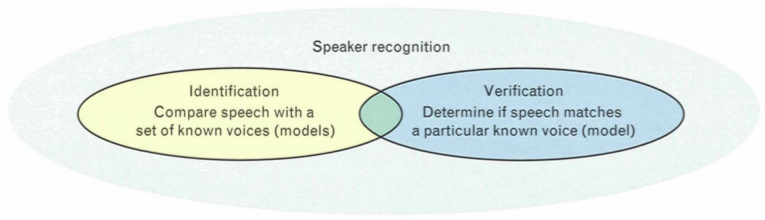
\includegraphics[width=0.75\textwidth]{speaker-recognition}
\end{figure}
\end{frame}

\begin{frame}
\frametitle{Dependência de texto}
\begin{description}
    \item[Com] Teste $\in$ Treinamento
    \pause
    \begin{itemize}
        \item Diversos graus de dependência
        \item Teste $\not\in$ Treinamento $\implies$ Retreinamento
        \pause
    \end{itemize}
    \item[Sem] Teste $\neq$ Treinamento
    \pause
    \begin{itemize}
        \item Características não textuais
        \item Presentes em diferentes sotaques e até \emph{gibberish}
        \pause
    \end{itemize}
    \item Este trabalho é focado em reconhecimento de locutor \textbf{independente de texto}
\end{description}
\end{frame}

\subsection{Modelos de Mistura Gaussiana}

\begin{frame}
\frametitle{Modelos de Mistura Gaussiana}
\begin{description}
    \item[GMM] \textbf{Combinação} de Gaussianas
    \pause
    \item[UBM] GMM gerado por diversas \textbf{locuções de fundo}
    \pause
    \item[AGMM] GMM \textbf{adaptado} a partir de um UBM
    \pause
    \item[FGMM] GMM utilizando \textbf{Fractional Covariance Matrix} (FCM)
\end{description}
\end{frame}

\subsection{Objetivos}

\begin{frame}
\frametitle{Objetivos}
\begin{description}
    \item Implementar sistemas de reconhecimento de locutor e analizar:
    \pause
    \begin{itemize}
        \item Taxas de \textbf{sucesso} para identificação
        \pause
        \begin{itemize}
            \item Diferentes tamanhos de mistura ($M$)
            \item Diferentes tamanhos de características ($\boldsymbol{\Delta}$)
            \pause
        \end{itemize}
        \item Comparar identificações utilizando GMM e FGMM
        \pause
        \item Taxas de \textbf{falsa detecção} e \textbf{falsa rejeição} para verificação
        \pause
        \begin{itemize}
            \item Diferentes tamanhos de mistura ($M$)
            \item Diferentes tamanhos de características ($\boldsymbol{\Delta}$)
            \pause
        \end{itemize}
        \item Comparar verificações utilizando GMM e AGMM
    \end{itemize}
\end{description}
\end{frame}